%!TEX root = pcp.tex

\chapter{Introduction}
\label{sec:introduction}

\section{Coloring}

Needless to say, graphs are widely used for modeling different scenarios in multiple areas of expertise, as well as for solving problems on those scenarios by translating them into well-known problems. 

One of those problems is the graph coloring problem, which consists in assigning a color to each node in a graph, with the constraint that two adjacent nodes must not have the same color. The objective is to generate a valid coloring using the minimum number of colors.

One of the most famous real life problems which led to the graph coloring problem was the \textit{4 colors problem}. In 1852, the question of whether any planar map could be colored using only four colors, in such a way that no two regions sharing a border had the same color, was posed. Modeling neighbour regions as adjacent nodes in a planar graph led to the planar graph coloring problem, which was eventually generalized into coloring a generic graph.

Graph coloring is widely used in multiple applications, such as schedule assignment to solve time incompatibilities, assignment of radio frequencies to prevent interference between neighboring radios, or even assigning variables to registers during the flow of a program.

The coloring of a graph is defined formally as a function that, given an input graph $G = <V,E>$, being $V$ the set of nodes and $E$ the set of undirected edges, assigns each node $v \in V$ to a natural number which represents a color, such that no two adjacent nodes have the same color. A \textit{k-coloring} is an assignment which uses exactly $k$ different colors.

\begin{figure}[h]
	\centering
	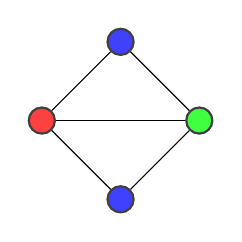
\begin{tikzpicture} 
		[n/.style= {minimum size=3mm,thick,circle,draw=black!75}] 
		
		\node[n,fill=red!75] (n0) at ( 0,0) {}; 
		
		\node[n,fill=blue!75] (n1) at ( 1,1) {}
			edge [-]	(n0)
		;

		\node[n,fill=green!75] (n2) at ( 2,0) {}
			edge [-]	(n1)
			edge [-]	(n0)
		;

		\node[n,fill=blue!75] (n3) at ( 1,-1) {}
			edge [-]	(n2)
			edge [-]	(n0)
		;
		
	\end{tikzpicture} 
\caption{Sample 3-coloring of a diamond graph.}
	\label{fig:samplecoloring}
\end{figure}

This problem has been proved to be \textit{NP-Complete}, and has been widely studied in the literature, being approached both by heuristic and exact methods for its resolution.

\subsection*{Previous Work}

Simplest heuristic approaches consist in greedy algorithms, using different criteria such as \textit{largest-first} \cite{welsh1967upper}, \textit{smallest-last} \cite{matula1972graph} or \textit{degree of saturation} \cite{brelaz1979new}. While the first two rely on a static ordering based on the degree of each node, the last one uses a dynamic ordering based on the number of different colors being used in the neighbourhood of each vertex.

These criteria may also be used in implicit enumeration techniques, which enumerate the possible colorings in the order determined by the chosen criteria. Using a good strategy is vital for finding good solutions as soon as possible, therefore pruning a great number of colorings. The implicit solution tree may be traversed in a BFS, DFS or best bound fashion. All these algorithms eventually find the optimal solution for the problem.

The \textsc{dsatur} enumeration algorithm proposed in \cite{brelaz1979new} has proven to be one of the most efficient implicit enumeration methods for the coloring problem, having several improvements such as \cite{sewell1996improved}.

More complex heuristic algorithms, using different metaheuristics, have also been used for the coloring problem.

There is also extensive work using integer linear programming formulations for the coloring problem by using different models:
\begin{itemize}
\item{In \cite{mehrotra1996column} a column generation approach is used based on an independent set formulation of the problem, in which a binary variable $x_S$ defines whether the independent set $S$ is given a color label or not; this formulation requires a variable for each possible color class in the graph.}
\item{An ILP model for acyclic orientations with path constraints is presented in \cite{figueiredo2005acyclic} and then applied to solve the vertex coloring problem.}
\item{The representatives model presented in \cite{campelo2004cliques} and \cite{campelo2008asymmetric} uses $x_{uv}$ variables which determine whether vertex $v$ \textit{represents} color $u$; having exactly one node represent each color class allows easy symmetry breaking.}
\item{In \cite{mendez2006branch,mendez2008cutting} both branch-and-cut and cutting planes algorithms were developed for a standard formulation of the problem, using $x_{ij}$ variables to specify whether node $i$ used color $j$, and $w_j$ variables as witnesses to whether color $j$ was in use. Several symmetry breaking constraints were added to the model to ensure a fast resolution.}
\end{itemize}

\section{Routing and Wavelength Assignment in WDM Networks}

A Wavelength Division Multiplexed (WDM) optical network consists in a network in which links are optical fibers capable of transmitting a specified number of different wavelengths. The Routing and Wavelength Assignment (RWA) problem consists in, given a desired set of connections between pairs of nodes, establish routes between those nodes using the network's links.

Every route is composed by a set of consecutive lightpaths. A lightpath is defined as a point to point connection between two adjacent nodes in the network using a certain wavelength. Although there are networks in which the nodes are capable of transforming wavelengths within the same route, we will assume that every route uses the same wavelength across all of its lightpaths; this restriction is known as the \textit{wavelength continuity constraint}.

The second restriction to be satisfied is the \textit{wavelength clash constraint} which imposes that different lightpaths in the same physical link must have different wavelengths. Together with the previous constraint, it is implied that two different routes that share at least one physical link must use different wavelengths.

In the offline or static version of the RWA problem, the set of connections to be established is known beforehand. The counterpart of this version is the \textit{dynamic} RWA in which connections must be satisfied as they are requested in an online fashion. In this work we will take only the former version into consideration.

The goal of the min-RWA is to minimize the number of different wavelengths required to establish all the routes desired. Note that there are multiple criteria that can be used to evaluate the quality of a set of routes, such as the number of lightpaths used for each route, or generating particular traffic patterns. In this work we will be focusing only in optimizing the number of wavelengths.

\section*{Previous Work}

Initial techniques to solve the min-RWA problem as a two-stage problem, such as \cite{hyytia14wavelength}, pick a single route for every connection using shortest-path algorithms and then use different heuristics to solve a standard coloring problem in the assignment stage. In \cite{manohar2002routing} the shortest-path routing solution is replaced by a maximum edge disjoint path solution in order to reduce conflicts between routes.

Other approaches to the problem tackle the routing and wavelength assignment as a single problem, without decomposing it in two separate phases. In \cite{skorin2007routing}, for example, bin packing heuristic algorithms are used to handle the problem, whereas \cite{noronha2007random} embeds this heuristic into a genetic evolutionary framework.

An exact approach using an integer programming formulation with column generation is used in \cite{lee2002optimization}, which solves both the routing and the wavelength assignment problems in the same formulation.

\section{Partitioned graph coloring problem}

A \textit{partitioned graph} is defined as a tuple $G = <V,E,P>$ of $n$ vertices, $m$ edges and $q$ partitions respectively. The set $P$ contains $P_1, \ldots ,P_q$ sets of nodes which constitute a partition of $V$. Therefore, for every node $v \in V$, there is exactly one $P_k \in P$ such that $v \in P_k$, and every $P_i \in P$ is nonempty.

The partitioned coloring problem is defined as an assignment of colors to the nodes of the graph $G$, with the restriction that no two adjacent nodes may have the same color, but requiring only one node per partition to be colored. Once again, the goal is to minimize the number of colors required.

\begin{figure}[h]
	\centering
	\begin{tikzpicture} 
		[n/.style= {minimum size=3mm,thick,circle,draw=black!75}] 
		
		\node[n,fill=black!25] (n0) at ( 0,0) {}; 
		
		\node[n,fill=blue!75] (n1) at ( 1,1) {}
			edge [-]	(n0)
		;

		\node[n,fill=black!25] (n2) at ( 4,0) {}
			edge [-]	(n1)
			edge [-]	(n0)
		;

		\node[n,fill=blue!75] (n3) at ( 3,-1) {}
			edge [-]	(n2)
			edge [-]	(n0)
		;
		
			\begin{pgfonlayer}{background} 
				\node [fill=black!10,circle,fit=(n0) (n1),label=170:$P_1$] {}; 
				\node [fill=black!10,circle,fit=(n2) (n3),label=350:$P_2$] {}; 
			\end{pgfonlayer}
		
	\end{tikzpicture} 
\caption{Sample 1-coloring of a partitioned diamond graph.}
	\label{fig:samplepartitionedcoloring}
\end{figure}

\subsection*{Complexity}

It is easy to see that when $|P_i| = 1\ \forall P_i \in P$, this is, there is a single node per partition, the partitioned coloring problem is equivalent to the standard graph coloring problem previously mentioned. In terms of complexity classes, PCP belongs to the same class as the standard coloring problem.

\begin{theorem}
The decision version of PCP is NP-Complete.
\end{theorem}

\begin{proof}
We will prove NP-Completeness by proving both belonging to NP and NP-Hard classes.

\begin{itemize}
\item{\textit{NP:} Given an input partitioned graph $G = <V,E,P>$ and an assignment of colors for a subset of nodes, checking that the number of colors used is $k$ is trivial, and a simple algorithm such as \ref{alg:pcpvalidity} can easily check the validity of the coloring in polynomial time.}
\item{\textit{NP-Hard:} Any instance of standard graph $k-coloring$ can be converted to an instance of PCP by partitioning the initial graph $G$ in such a way that every partition contains a single node. The solution to the original $k-coloring$ problem is the same as the solution to the constructed \PCP{}. Since standard coloring is NP-Hard, this implies that PCP is NP-Hard as well.}
\end{itemize}

\end{proof}

\begin{algorithm}
\caption{Polynomial time algorithm for checking validity of a partition coloring}
\label{alg:pcpvalidity}
\begin{algorithmic}

\FORALL{partition $p$ in $P$}
	\FORALL{node $v$ in $p$}
		\IF {$v$ has a color $j$ assigned}
			\STATE mark $p$ as colored
			\FORALL {neighbour $u$ to $v$}
				\IF{$u$ has the same color assigned as $v$}
					\RETURN false
				\ENDIF	
			\ENDFOR
		\ENDIF
	\ENDFOR
	\IF {no node $v$ in $P$ was colored}	
		\RETURN false
	\ENDIF	
\ENDFOR

\end{algorithmic}
\end{algorithm}

\subsection*{Resolution of min-RWA using PCP}

There are multiple methods, both heuristic and exact, for solving the min-RWA problem. Some of them handle both the routing and the wavelength assignment as the same problem, whereas other methods, such as the one proposed in \cite{Li00thepartition}, use a two-phase approach: a routing phase and an assignment phase.

In the routing phase, a set of potential routes is generated for every pair of nodes to be connected, mostly using shortest-path criteria.

The assignment phase then requires to pick a route from the set of candidates for every connection. The route chosen is assigned a wavelength, in such a way that no pair of routes that share a physical link have the same wavelength. This phase can be transformed into an instance of \PCP{}.

A partitioned graph $G$ can be constructed in the following way:
\begin{itemize}
\item{Every potential route generated in the routing phase is represented by a node $v \in V$.}
\item{Nodes belong to the same partition iff the routes they represent satisfy the same connection request.}
\item{An edge between two nodes $u,v$ is created if the routes share any physical link.}
\end{itemize}

\begin{figure}[h]
	
	\centering
	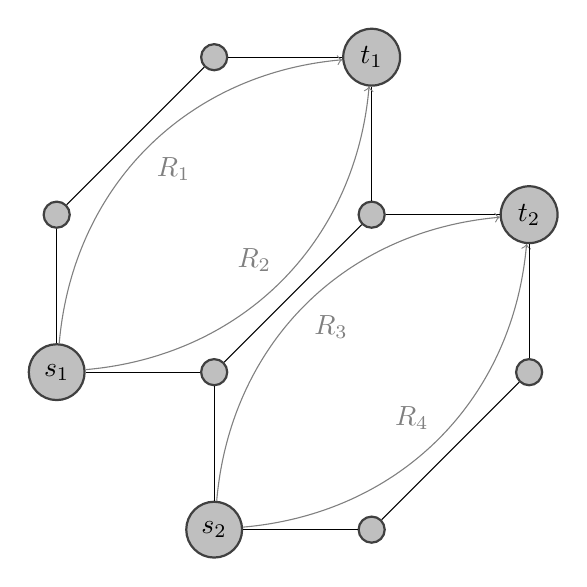
\begin{tikzpicture} 
		[bend angle=40,
		n/.style= {minimum size=3mm,thick,circle,draw=black!75,fill=black!25}] 
		
		\node[n] (n0) at ( 0,0) {$s_1$}; 
		
		\node[n] (n1) at ( 0,2) {}
			edge [-]	(n0)
		;

		\node[n] (n2) at ( 2,4) {}
			edge [-]	(n1)
		;
		
		\node[n] (n4) at ( 2,0) {}
			edge [-]	(n0)
		;
		
		\node[n] (n5) at ( 4,2) {}
			edge [-]	(n4)
		;
		
		\node[n] (n3) at ( 4,4) {$t_1$}
			edge [-]	(n2)
			edge [-]	(n5)
			edge [<-, bend right, draw=black!50] node[auto] {\textcolor{black!50}{$R_1$}} 	(n0)
			edge [<-, bend left, draw=black!50] node[auto,swap] {\textcolor{black!50}{$R_2$}} (n0)
		;
		
		\node[n] (n6) at ( 2,-2) {$s_2$}
			edge [-]	(n4)
		;
		
		\node[n] (n7) at ( 6,2) {$t_2$}
			edge [-]	(n5)
			edge [<-, bend right, draw=black!50] node[auto] {\textcolor{black!50}{$R_3$}}  (n6)
			edge [<-, bend left, draw=black!50]	node[auto,swap] {\textcolor{black!50}{$R_4$}} (n6) 
		;
		
		\node[n] (n8) at ( 4,-2) {}
			edge [-]	(n6)
		;

		\node[n] (n9) at ( 6,0) {}
			edge [-]	(n8)
			edge [-]	(n7)
		;
		
	\end{tikzpicture} 

		\caption{Sample network in which connections $s_1 \rightarrow t_1$ and $s_2 \rightarrow t_2$ are to be implemented. Potential routes $R_1, R_2$ are proposed for the first, while routes $R_3, R_4$ are proposed for the second one. The corresponding partitioned graph is presented in figure \ref{fig:solvedsamplerouting}.}
		
		\label{fig:samplerouting}
	\end{figure}
	
\begin{figure}[h]

		\centering	
		\begin{tikzpicture} 
			[n/.style= {minimum size=3mm,thick,circle,draw=black!75}] 

			\node[n,fill=blue!25] (n0) at ( 0,0) {$R_1$}; 

			\node[n,fill=black!25] (n1) at ( 0,2) {$R_2$};

			\node[n,fill=black!25] (n2) at ( 5,0) {$R_3$}
				edge [-]	(n1)
			;

			\node[n,fill=blue!25] (n3) at ( 5,2) {$R_4$};

				\begin{pgfonlayer}{background} 
					\node [fill=black!10,circle,fit=(n0) (n1),label=170:$s_1 \rightarrow t_1$] {}; 
					\node [fill=black!10,circle,fit=(n2) (n3),label=350:$s_2 \rightarrow t_2$] {}; 
				\end{pgfonlayer}

		\end{tikzpicture} 
	
		\caption{Conflicts partitioned graph for network from figure \ref{fig:samplerouting}. Routes $R_1$ and $R_2$ satisfy the same connection request, as such, they are contained in the same partition; same happens for $R_3$ and $R_4$. Since routes $R_2$ and $R_3$ share a physical link, the corresponding nodes are adjacent to prevent that they are assigned the same frequency. A 1-coloring, which assigns the same label to $R_1$ and $R_4$ is shown, and the corresponding lightpaths generated are shown in figure \ref{fig:solvedsampleroutingnetwork}.}

		\label{fig:solvedsamplerouting}
\end{figure}

\begin{figure}[h]
	\centering
	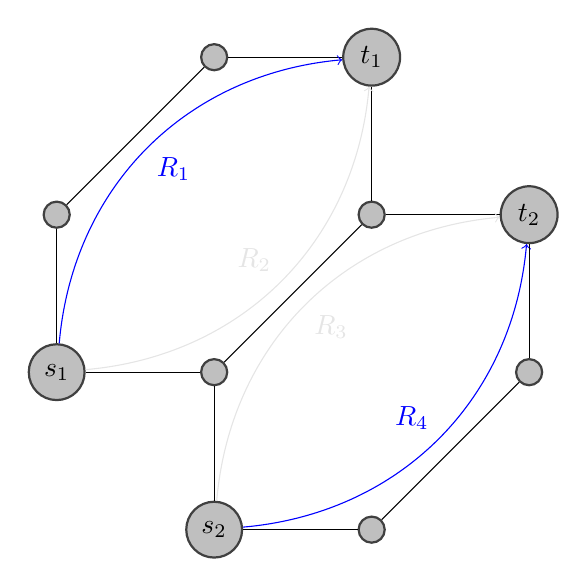
\begin{tikzpicture} 
		[bend angle=40,
		n/.style= {minimum size=3mm,thick,circle,draw=black!75,fill=black!25}] 
		
		\node[n] (n0) at ( 0,0) {$s_1$}; 
		
		\node[n] (n1) at ( 0,2) {}
			edge [-]	(n0)
		;

		\node[n] (n2) at ( 2,4) {}
			edge [-]	(n1)
		;
		
		\node[n] (n4) at ( 2,0) {}
			edge [-]	(n0)
		;
		
		\node[n] (n5) at ( 4,2) {}
			edge [-]	(n4)
		;
		
		\node[n] (n3) at ( 4,4) {$t_1$}
			edge [-]	(n2)
			edge [-]	(n5)
			edge [<-, bend right, draw=blue!100] node[auto] {\textcolor{blue!100}{$R_1$}} 	(n0)
			edge [<-, bend left, draw=black!10] node[auto,swap] {\textcolor{black!10}{$R_2$}} (n0)
		;
		
		\node[n] (n6) at ( 2,-2) {$s_2$}
			edge [-]	(n4)
		;
		
		\node[n] (n7) at ( 6,2) {$t_2$}
			edge [-]	(n5)
			edge [<-, bend right, draw=black!10] node[auto] {\textcolor{black!10}{$R_3$}}  (n6)
			edge [<-, bend left, draw=blue!100]	node[auto,swap] {\textcolor{blue!100}{$R_4$}} (n6) 
		;
		
		\node[n] (n8) at ( 4,-2) {}
			edge [-]	(n6)
		;

		\node[n] (n9) at ( 6,0) {}
			edge [-]	(n8)
			edge [-]	(n7)
		;
		
	\end{tikzpicture} 
		
		\caption{Solution for the network presented in figure \ref{fig:samplerouting} using the coloring obtained in \ref{fig:solvedsamplerouting}. Since $R_1$ and $R_4$ were the colored nodes, using the same label, then those are the routes established and lightpaths using that label are created to satisfy the connection requests.}
		\label{fig:solvedsampleroutingnetwork}
	\end{figure}

Each wavelength is represented as a color. The problem then consists in coloring a single node within each partition, this is, assigning a wavelength to a single route from the set of candidates for each connection request. The fact that two nodes may not be colored if they are adjacent guarantees  that no wavelength conflicts may occur between two different lightpaths in the same link.

An example is shown in figures \ref{fig:samplerouting}, \ref{fig:solvedsamplerouting} and \ref{fig:solvedsampleroutingnetwork}.

In this work we will focus on finding an exact solution for the partitioned coloring problem, using a branch and cut algorithm based on a generalization of the coloring model proposed in \cite{mendez2006branch,mendez2008cutting}.

\subsection*{Previous work}

In \cite{Li00thepartition}, two groups of heuristics were developed for solving the \PCP{}: one-step and two-step. The former consists in picking the easiest node to color in every partition, and then picking the hardest one from that set using different criteria (largest-first, smallest-last, color-degree); the latter makes an initial pass picking the easiest nodes in every partition and inducing a non-partitioned graph, onto which a standard heuristic is applied in a second stage.

In \cite{noronha2006routing} the one-step color-degree constructive heuristic is used in a tabu search approach, TS-PCP. Routes are generated in an initial stage using a $k$-EDR constructive procedure, based on the maximum edge disjoint path heuristic by \cite{kleinberg1996approximation}, and the resulting partitioned coloring problem is solved with TS-PCP.

Due to the complexity of the problem, most of the work on PCP is composed by heuristic approaches. However, in \cite{frota2010branch}, a branch and cut algorithm is devised, using an integer linear programming model based on the asymmetric representatives formulation for the standard coloring problem, presented in \cite{campelo2004cliques} and \cite{campelo2008asymmetric}.

\section{Objective of this work}

A common approach for obtaining exact solutions to complex combinatorial optimization problems is to model them as integer linear programming problems, and solve them using branch and bound, cutting planes or branch and cut algorithms, among others. 

Therefore, the objective of this work will be to develop a branch and cut algorithm for solving the partitioned coloring problem, by modelling it as an integer linear programming problem, with a generalization of the standard coloring model presented in \cite{mendez2006branch,mendez2008cutting}. 

We will be using \textsc{cplex} as a branch and cut framework and introduce custom initial heuristics, cutting planes, primal heuristics and branching strategies, designed specifically for this problem, and evaluate their performance against the default implementation provided by \textsc{cplex}.

This work is structured in seven chapters. In chapter \ref{sec:model} we present different models for representing an instance of \PCP{}, starting with a basic model that captures all necessary restrictions, for later strengthening it by modifying the constraints with stronger ones or introducing new ones, such as symmetry breaking constraints.

Chapter \ref{sec:ineqs} dwelves deeper into the polyhedron defined in the previous chapter by presenting valid inequalities derived for \PCP{}. These inequalities will be later applied as cutting planes in both cutting planes and branch and cut algorithms.

Alternative algorithms for solving the problem are presented in chapter \ref{sec:heur}. We present enumeration algorithms for solving the standard coloring problem, and generalize them for partition coloring, focusing in the \textsc{dsatur} algorithm \cite{brelaz1979new} and its generalization. These algorithms will be adapted to be used as initial and primal heuristics during the branch and cut process.

The implemented branch and cut algorithm is presented in chapter \ref{sec:bnc}, where we present the general structure for cutting plane, branch and bound and branch and cut algorithms, as well as different components of a branch and cut (separation heuristics, initial heuristics, primal heuristics, branching strategies, node selection strategies) and how we implemented them for dealing with the \PCP{}.

This implementation is then tested in chapter \ref{sec:results}. Given a test suite of binomial, powerlaw cluster and \textsc{dimacs} challange graphs, we first evaluated multiple configurations for all of the different components, starting by choosing a model to be used in the algorithm, and testing the effectiveness of the different heuristics and strategies with different parameterizations. We then test the performance of the algorithm, once we have all parameters fixed, against a fresh test suite and report the obtained MIP gap.

Finally, in chapter \ref{sec:conclusions}, we sum up the work achieved, draw conclusions from it and present possible future research lines.

\section{Definitions}
\label{subsec:intro:definitions}

In this section we will define all concepts and conventions to be used throughout this work: 

\begin{itemize}
	\defitem{Colors}{The set of valid color labels $C = \{1, \ldots, c\}$, where $c$ may be any upper bound to the chromatic number of the graph, such as $n$.}
	\defitem{Graph}{Defined as tuple $<V,E>$ where $V$ is the set containing the $n$ nodes and $E$ contains the $m$ undirected edges.}
	\defitem{Partitioned Graph}{Defined as tuple $<V,E,P>$, being $V$ and $E$ the same sets as above, and $P$ the set of $P_1, \ldots, P_q$ partitions of $V$.}
	\defitem{Partition function}{For every node $v$ in a partitioned graph, $p(v)$ returns the partition that contains that node.}
	\defitem{Neighbourhood}{$N(v)$ is the set of nodes in $V$ adjacent to node $v$.}
	\defitem{Partition Neighbourhood}{$N_P(v)$ is the set of partitions that contain at least one node adjacent to $v$.}
	\defitem{Degree}{$\delta(v)$ is the cardinal of the neighbourhood of $v$.}
	\defitem{Partition Degree}{$\delta_P(v)$ is the cardinal of the partition neighbourhood of $v$.}
	\defitem{Color Degree}{Number of different colors used in $N(v)$ for a node $v \in V$; also degree of saturation.}
	\defitem{Extended Clique}{Subset of $V$ such that for every pair of nodes $u,v$, either $u$ is adjacent to $v$ or $u$ and $v$ are contained in the same partition.}
	\defitem{Component Independent Set}{Subset of $V$ such that for every pair of nodes $u,v$, $u$ is not adjacent to $v$ and they belong to different partitions.}
	\defitem{Partition Graph}{The \textit{partition graph} $G'$ of a partitioned graph $G$ is a standard graph $G'=<V',E'>$ in which every node $v'_k \in V'$ corresponds to a partition $P_k \in P$, and two nodes $v'_i,v'_j \in V'$ are adjacent if and only if every node in $P_i$ in $G$ is adjacent to every node in $P_j$.}
\end{itemize}